% !TEX root = HW5.tex
\newcommand{\studSolAA}{
	%%%%%%%%%%%%%%%%%%%%%%%%%%%%%%%%%%%%
	%%
	%%.   YOUR SOLUTION FOR PROBLEM A BELOW THIS COMMENT
	%%
	%%%%%%%%%%%%%%%%%%%%%%%%%%%%%%%%%%%%
	\\For multiclass classification: ii. Labels: each of the different species that can be recognized.\\
	For binary classification: iii. Labels: approved or not-approved.
}

\newcommand{\studSolAB}{
	%%%%%%%%%%%%%%%%%%%%%%%%%%%%%%%%%%%%
	%%
	%%.   YOUR SOLUTION FOR PROBLEM A BELOW THIS COMMENT
	%%
	%%%%%%%%%%%%%%%%%%%%%%%%%%%%%%%%%%%%
	\\For 1-vs-all: $n - 1$ classifiers.\\
	For 1-vs-1: 
	\[
		\frac{n\left(n-1\right)}
		{2}
	\]
}

\newcommand{\studSolAC}{
	%%%%%%%%%%%%%%%%%%%%%%%%%%%%%%%%%%%%
	%%
	%%.   YOUR SOLUTION FOR PROBLEM A BELOW THIS COMMENT
	%%
	%%%%%%%%%%%%%%%%%%%%%%%%%%%%%%%%%%%%
	Let $c_{i, j}$ be the classifier for classes $i$ and $j$, $i, j = 0, 1, ..., K - 1, i < j$. Note that we only have one training example for each class so every example will be in the margin boundary for every $c_{i, j}$.  Below there is a plot of one of these classifiers ignoring all the dimensions that have zero for both points. The marked points are the support vectors and the green line is the decision boundary. It is easy to see that $w$ for this classifier is $(-1, 1)$ (to a scale). \\
	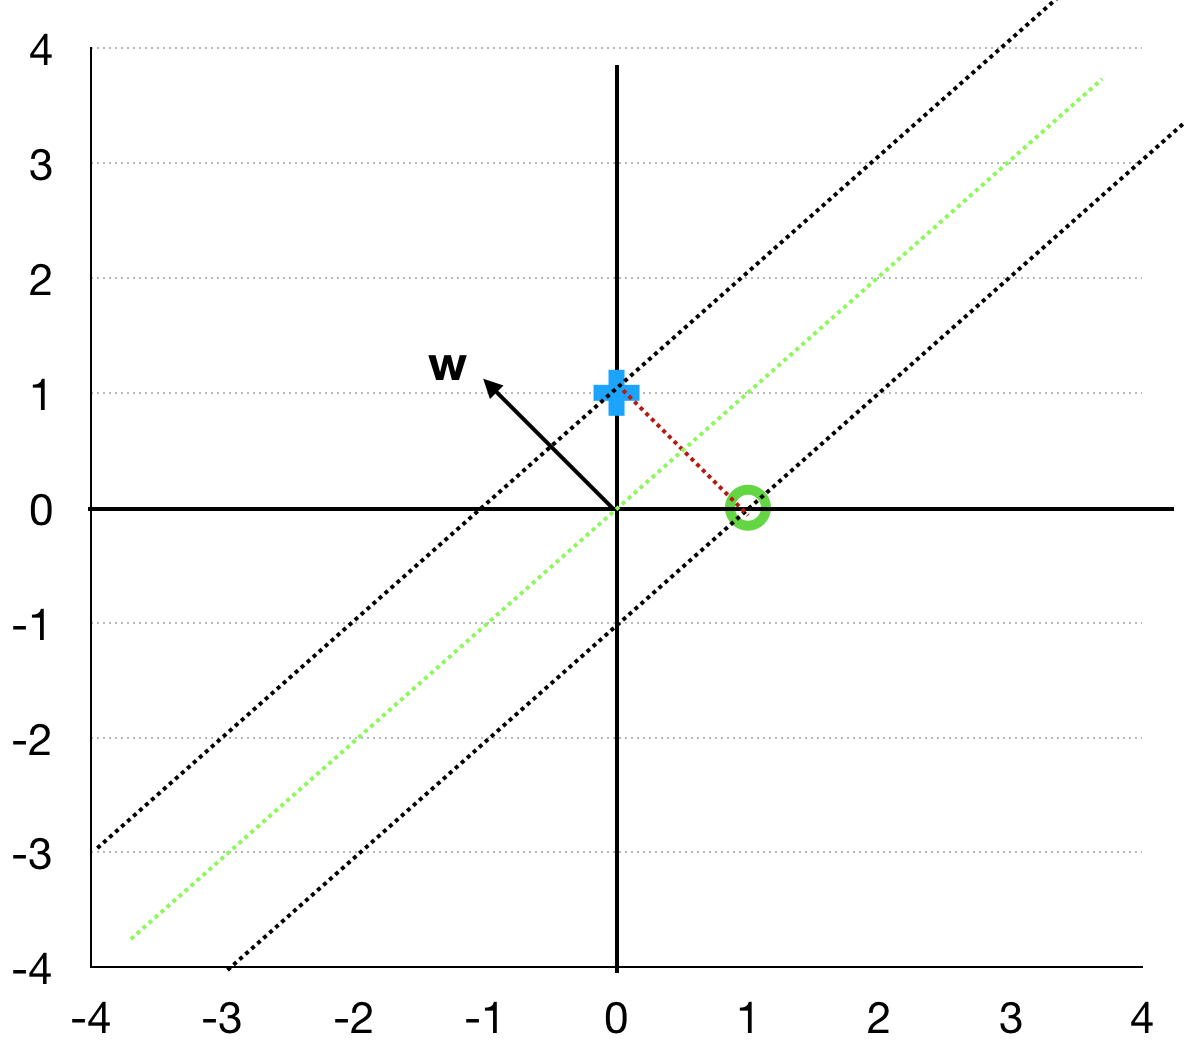
\includegraphics[scale=0.4]{svm.png}
	
	Now consider a test example $x = (x_1, x_2, ..., x_n)$; when tested against $c_{i, j}$ we only care about the components $i, j$ of $x$. In particular, if $x_i > x_j$ then $x$ will be classified as class $i$.\\
	
	Since in particular case is symmetric, e.g. we can take any permutation of the classes and the problem won't change, without loss of generality lets assume that 
	\[x_1 \ge x_2 \ge ... \ge x_n\]
	Note that we can actually assume strict inequality since we are ignoring points in decision boundaries. So,
	\[ x_1 > x_2 > ... > x_n \]
	
	This means that $c_{1, 2}, c_{1, 3}, ..., c_{1, n}$ will all vote for class 1. So \textit{at least} $n-1$ classifiers will vote for class 1. Now note that $c_{2, 3}, c_{2, 4}, ..., c_{2, n}$ will all vote for class 2 so there are at least $n-2$ votes for class 2. By doing this for all $i$ in $c_{i, j}$ we can see that there are exactly $n-i$ classifiers that will vote for class $i$. Therefore, there are \textbf{no} regions in the Euclidean space that will receive the same number of majority votes for more than one class other than the decision boundaries.
}

\newcommand{\constraint}[1]{w_{y^{(#1)}} \phi\left(x^{(#1)}\right) - w_{\hat{y}} \phi\left(x^{(#1)}\right)}
\newcommand{\studSolBA}{
	
	%%%%%%%%%%%%%%%%%%%%%%%%%%%%%%%%%%%%
	%%
	%%.   YOUR SOLUTION FOR PROBLEM A BELOW THIS COMMENT
	%%
	%%%%%%%%%%%%%%%%%%%%%%%%%%%%%%%%%%%%
	Let $w_1, w_2$ be the weights of the classifier for class 0, $w_3, w_4$ for class 1, and, $w_5, w_6$ for class 2.\\
	
	Let's now rewrite the constraints using the given setup. \\
	For $i = 1, \hat{y} = 1$: \\
	\begin{align*}
		\constraint{1} &= 
			\left( 0w_1 + (-1)w_2 \right) - 
			\left( 0w_3 + (-1)w_4 \right)\\
		&= -w_2 + w_4\\
		& \ge 1 - \xi^{(1)}
	\end{align*}
	
	Similarly, for\\
	\[ i = 1, \hat{y} = 2 \rightarrow -w_2 + w_6 \ge 1 - \xi^{(1)} \]
	\[ i = 2, \hat{y} = 0 \rightarrow w_3 - w_1 \ge 1 - \xi^{(2)} \]
	\[ i = 2, \hat{y} = 2 \rightarrow w_3 - w_5 \ge 1 - \xi^{(2)} \]
	\[ i = 3, \hat{y} = 0 \rightarrow w_6 - w_2 \ge 1 - \xi^{(3)} \]
	\[ i = 3, \hat{y} = 1 \rightarrow w_6 - w_4 \ge 1 - \xi^{(3)} \]
	
	We know that $||w||^2 = w_1^2 + w_2^2 + w_3^2 + w_4^2 + w_5^2 + w_6^2$ so the objective function can be rewritten as 
	\[
		\min_{w_1, ..., w_6, \xi^{(i)} \ge 0} \frac{C}{2}\left(	
			w_1^2 + w_2^2 + w_3^2 + w_4^2 + w_5^2 + w_6^2
		\right) + \sum_{i = 1}^n \xi^{(i)}
	\]
	s.t. the six constraints above.
}

\newcommand{\studSolBB}{
	%%%%%%%%%%%%%%%%%%%%%%%%%%%%%%%%%%%%
	%%
	%%.   YOUR SOLUTION FOR PROBLEM A BELOW THIS COMMENT
	%%
	%%%%%%%%%%%%%%%%%%%%%%%%%%%%%%%%%%%%
	By solving for $\xi^{(i)}$ on each of the constraints and taking the max for each of the $\xi$ we have that the function can be written as
	
	\begin{multline*}
		\min_{w_1, ..., w_6} \frac{C}{2}\left(	
			w_1^2 + w_2^2 + w_3^2 + w_4^2 + w_5^2 + w_6^2
		\right)\\
		+ \max \left( 
				1 + w_2 - w_4,
				1 + w_2 - w_6
			\right)\\
		+ \max \left(
				1 + w_1 - w_3,
				1 + w_5 - w_3
			\right)\\
		+ \max \left(
				1 + w_2 - w_6,
				1 + w_4 - w_6
			\right)\\
	\end{multline*}
}

\newcommand{\studSolBC}{
	%%%%%%%%%%%%%%%%%%%%%%%%%%%%%%%%%%%%
	%%
	%%.   YOUR SOLUTION FOR PROBLEM A BELOW THIS COMMENT
	%%
	%%%%%%%%%%%%%%%%%%%%%%%%%%%%%%%%%%%%
	Note that in 2(b) $\max \left(
				1 + w_1 - w_3,
				1 + w_5 - w_3
			\right)$ does not depend on $w_2$ so its derivative will be zero.\\
	Also note that the partial w.r.t $w_2$ of $\max \left( 
				1 + w_2 - w_4,
				1 + w_2 - w_6
			\right)$ will be 1.\\
	We now need to plug $w_t$ in the 
	\[
		\max \left(
				1 + w_2 - w_6,
				1 + w_4 - w_6
			\right) = 
		\max \left( 1 + 1 - (-1), 1 + 2 - (-1) \right)
	\]
	Since the second term is higher the partial w.r.t. $w_2$ of this term is zero.
	Finally we have that:
	\[
		\frac{\partial F}
		{\partial w_2}	 = 
			Cw_2 + 1 + 0 + 0 = 
			C + 1
	\]
}

\newcommand{\studSolBD}{
	\newcommand{\wyhat}{1 + w_{\hat{y}}^\intercal \phi \left( x \right)}
	%%%%%%%%%%%%%%%%%%%%%%%%%%%%%%%%%%%%
	%%
	%%.   YOUR SOLUTION FOR PROBLEM A BELOW THIS COMMENT
	%%
	%%%%%%%%%%%%%%%%%%%%%%%%%%%%%%%%%%%%
	Lets start by remembering that the Chebyshev norm is given by
	\[
		||\mathbf{z}||_{\infty} =
		\lim_{p \rightarrow \infty} \left( \sum_{i} z_i^p \right)^{\frac{1}{p}} =
		\max_i \left( z_i \right)
	\]
	
	Since $f(z) = \exp(z)$ is a monotone function we have that
	\[
		\max_i(z_i) = 
		\ln \max_i \left( \exp \left( z_i \right) \right)
	\]
	
	Combining these two results it follows that
	\begin{align*}
		\max_{\hat{y}}\left( \wyhat \right) &= \ln \max_{\hat{y}} \left( \exp \left( \wyhat \right) \right)\\
		&= \ln \lim_{p 
			\rightarrow \infty} \left( 
				\sum_{\hat{y}}
					\exp \left( \wyhat \right)^p 
			\right)^{\frac{1}{p}}\\
		&= \lim_{p \rightarrow \infty}
			\ln \left( 
				\sum_{\hat{y}}
					\exp \left( \wyhat \right)^p 
			\right)^{\frac{1}{p}}\\
		&= \lim_{\epsilon \rightarrow 0} 
			\ln \left( 
				\sum_{\hat{y}}
					\exp \left( \wyhat \right)^{\frac{1}{\epsilon}} 
			\right)^\epsilon\\
		&= \lim_{\epsilon \rightarrow 0}
			\epsilon \ln
				\sum_{\hat{y}}
					\exp \left( \wyhat \right)^{\frac{1}{\epsilon}}\\
		&= \lim_{\epsilon \rightarrow 0}
			\epsilon \ln
				\sum_{\hat{y}}
					\exp \frac{1}{\epsilon} \left( \wyhat \right)\\
		&= \lim_{\epsilon \rightarrow 0}
			\epsilon \ln
				\sum_{\hat{y}}
					\exp \left( \frac{\wyhat}{\epsilon} \right) \blacksquare
	\end{align*}
}